\section {Reaching Definitions}
\setlength{\parindent}{0pt}
(Prepared by Sameer V. Pande)

\vspace{0.3cm}

Reaching definitions is a more-detailed dataflow analysis, which contains the "possible" definitions a variable can take at a program point, unlike available-expression analysis, which indicates the value that a variable definitely takes.
This is more fine-grained because it doesn't declare variable values as $\bot$ when a variable can potentially have more than one value (depending on the path taken to reach the point), unlike available-expression analysis.
\newline 
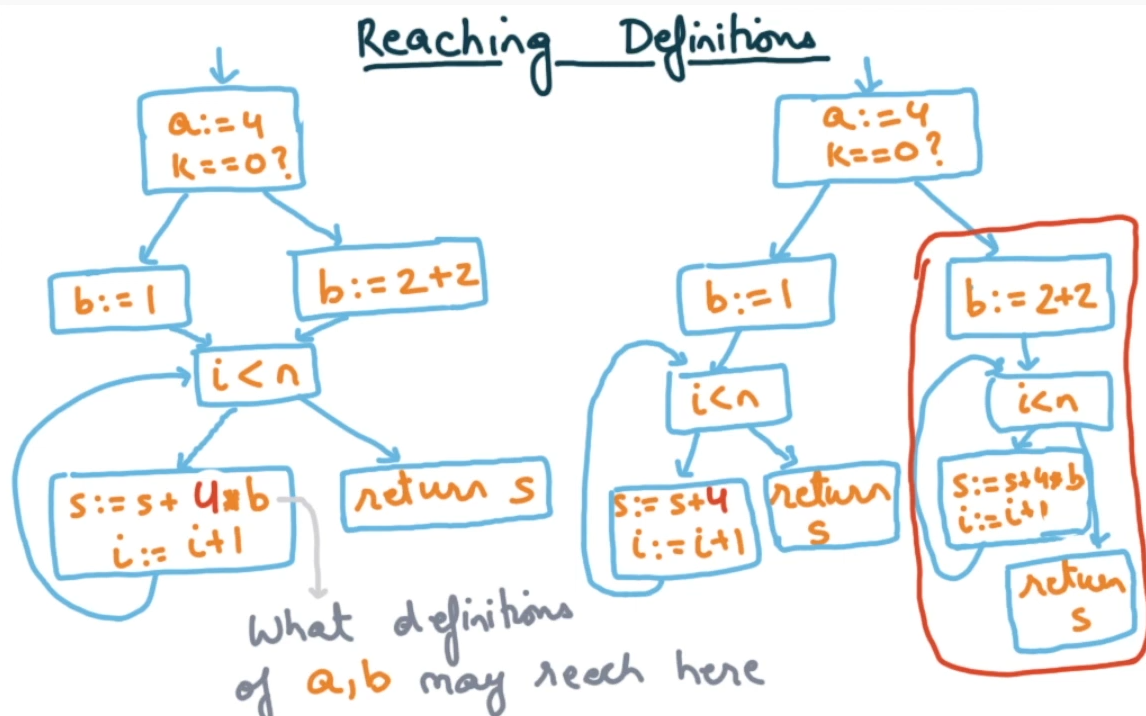
\includegraphics[scale=0.3]{images/90_1.png}

Consider the example above, and assume that program usually spends most of its execution time in the loop. In the loop, the variable "b" can have two values "1"/"y+z". If we use reaching-definitions analysis we can know that only two values of "b" are possible (one of which is a constant) and we can \textbf{specialize} the code (as seen in right-figure), by replicating the branch and specializing one of the branch on a constant value of b.

\subsection{Gen/Kill Sets and Meet for Reaching Definitions}
It is a forward dataflow analysis. Gen(S) of a statment S, contains all the new definitions generated by the S. And kill contains all definitions killed.
Hence for the example "S:x=y+z", Gen(S) = \{(x,y+z)\} and Kill(S) = \{(x,*)\}.
\newline
In reaching definitions the \textbf{meet operator is union}. Meet is union operator because we want the definitions which can reach the program point via \textbf{any} path. 

\subsection{Reaching Definitions vs Available Expressions}
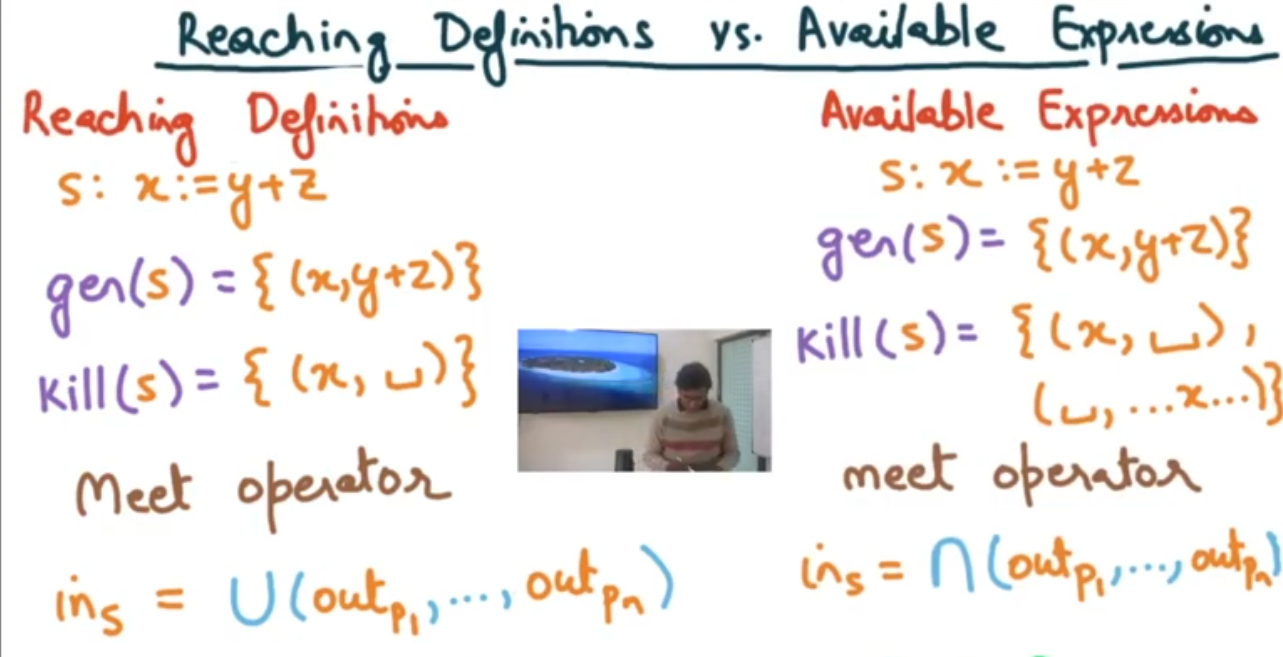
\includegraphics[scale=0.3]{images/90_2.png}
It is important to note that "Reaching-Defintions" is analysis involving definitions and "Available-Expressions" involves expressions.
From above figure, we can see that Gen() is very similar for both. But there are important differences in the following 
\begin{itemize}
    \item Kill Set: In addition to (x,*), available-expressions also kills (*, ...x...) i.e. all variables with values dependent on previous value of x. This is not present in reaching-defintions since we are only worried about "definitions", we don't have to deal with this case (where x also appears in rhs). 
    \item Meet Operator: The meet operator of reaching definitions is \textbf{union} because we want to consider \textbf{any} defintion of a varialbe that can reach at current program point \textbf{through any path}. 
    Whereas available-expressions requires the same expression to reach the current program point through \textbf{all possible paths}. Hence \textbf{intersection} is suitable for available expressions. 
\end{itemize}